\documentclass[11pt,a4paper]{article}

% ============================================================
%  SmartParking - Documentazione progetto TVSW
%  Compilare con: pdflatex main.tex  (due volte, per indice/riferimenti)
% ============================================================

\usepackage[utf8]{inputenc}
\usepackage[T1]{fontenc}
% Carica babel con sillabazione italiana se il pacchetto linguistico e'
% disponibile (caso normale su MacTeX/TeX Live completo); altrimenti
% carica babel senza opzione di lingua, cosi' il documento compila
% comunque (succede solo su installazioni minimali senza
% texlive-lang-italian, es. alcuni Linux "headless").
\IfFileExists{italian.ldf}{\PassOptionsToPackage{italian}{babel}}{}
\usepackage{babel}
\usepackage{graphicx}
\usepackage{tikz}
\usetikzlibrary{positioning,arrows.meta}
\usepackage{underscore} % permette di usare "_" nel testo normale senza errori
\usepackage{listings}
\usepackage{xcolor}
\usepackage{hyperref}
\usepackage{booktabs}
\usepackage{longtable}
\usepackage{amsmath}
\usepackage{amssymb}
\usepackage{geometry}
\usepackage{fancyhdr}
\usepackage{caption}
\usepackage{float}
\usepackage{parskip}
\geometry{margin=2.5cm}

\hypersetup{
    colorlinks=true,
    linkcolor=blue!50!black,
    citecolor=black,
    urlcolor=blue!50!black,
    pdftitle={SmartParking - Documentazione Progetto TVSW},
    pdfauthor={Francesco Tomasoni}
}

\pagestyle{fancy}
\fancyhf{}
\rhead{Francesco Tomasoni}
\lhead{SmartParking - TVSW}
\rfoot{\thepage}

% --- Stile per il codice sorgente (ASM / Java / YAML / shell) ---
\lstdefinestyle{code}{
    basicstyle=\ttfamily\footnotesize,
    breaklines=true,
    breakatwhitespace=false,
    frame=single,
    backgroundcolor=\color{black!5},
    keywordstyle=\color{blue!70!black}\bfseries,
    commentstyle=\color{green!40!black}\itshape,
    stringstyle=\color{orange!70!black},
    numbers=left,
    numberstyle=\tiny\color{gray},
    stepnumber=1,
    tabsize=4,
    showstringspaces=false
}
\lstset{style=code}

% --- Stile "terminale" (sfondo scuro, testo chiaro): per contratti JML e output CLI ---
\lstdefinestyle{terminal}{
    basicstyle=\ttfamily\footnotesize\color{green!45!white},
    backgroundcolor=\color{black!90},
    frame=single,
    rulecolor=\color{black},
    breaklines=true,
    breakatwhitespace=false,
    keywordstyle=\color{green!45!white},
    commentstyle=\color{green!70!white},
    stringstyle=\color{green!45!white},
    identifierstyle=\color{green!45!white},
    numbers=none,
    tabsize=4,
    showstringspaces=false,
    columns=fullflexible,
    keepspaces=true
}

% --- Stile "trascrizione LLM": riquadro chiaro, senza numeri di riga,
%     spezzabile su piu' pagine. Usato per riportare prompt e risposta
%     della rilettura critica del codice (Sezione analisi statica). ---
\lstdefinestyle{llm}{
    basicstyle=\ttfamily\scriptsize,
    backgroundcolor=\color{blue!4},
    frame=single,
    rulecolor=\color{black!35},
    breaklines=true,
    breakatwhitespace=false,
    numbers=none,
    tabsize=2,
    showstringspaces=false,
    columns=fullflexible,
    keepspaces=true,
    extendedchars=true,
    literate={à}{{\`a}}1 {è}{{\`e}}1 {é}{{\'e}}1 {ì}{{\`i}}1
             {ò}{{\`o}}1 {ù}{{\`u}}1 {È}{{\`E}}1 {'}{{'}}1
             {→}{{$\rightarrow$}}1 {–}{{--}}1
}

% ============================================================
%  Comando \screenshot{nomefile}{didascalia}{descrizione}
%
%  Se images/<nomefile>.png esiste, la include normalmente.
%  Altrimenti mostra un riquadro segnaposto con il nome del file
%  atteso e la descrizione di cosa deve mostrare lo screenshot,
%  cosi' il documento compila correttamente anche PRIMA di avere
%  tutte le immagini pronte. Basta salvare il file .png con il
%  nome giusto dentro docs/latex/images/ e ricompilare.
% ============================================================
\newcommand{\screenshot}[3]{%
    \begin{figure}[H]
        \centering
        \IfFileExists{images/#1.png}{%
            \includegraphics[width=0.85\textwidth]{images/#1.png}%
        }{%
            \fbox{\begin{minipage}{0.85\textwidth}
                \centering
                \vspace{1.5cm}
                {\bfseries\color{red} [SCREENSHOT MANCANTE: images/#1.png]}\\[0.5cm]
                \parbox{0.75\textwidth}{\centering\small #3}
                \vspace{1.5cm}
            \end{minipage}}%
        }
        \caption{#2}
        \label{fig:#1}
    \end{figure}
}

\title{\textbf{SmartParking} \\ \large Documentazione del progetto Testing e Verifica del Software}
\author{Francesco Tomasoni 1080980}
\date{A.A. 2025/2026}

\begin{document}

\maketitle
\thispagestyle{empty}

\tableofcontents
\newpage

% ATTENZIONE: l'ordine di inclusione non segue la numerazione dei nomi file.
% I file sono stati numerati secondo lo schema punteggi del progetto, mentre qui
% sono in ordine di lettura. Quindi 04_java.tex e' la Sezione 3, 05_testing.tex
% e' la Sezione 4 e 03_jml.tex e' la Sezione 5.
\section{Introduzione e requisiti}

\subsection{Descrizione del sistema}

SmartParking è un parcheggio automatico. Ci sono due sbarre, una in ingresso e una in
uscita, dei sensori che si accorgono quando arriva un'auto e un totem che legge che tipo
di utente è. I posti sono di due tipi: standard e riservati ai disabili. Nel modello ne
ho messo uno solo per tipo, altrimenti il model checker dopo esplode.
\\ \\
Gli utenti sono tre:

\begin{itemize}
\item \textbf{STD}: l'utente standard, è l'unico che paga;
\item \textbf{DISABILE}: ha il permesso, non paga e ha la precedenza sui posti riservati;
\item \textbf{ABBONATO}: ha l'abbonamento mensile e non paga.
\end{itemize}

Quando arriva un'auto il sistema la rileva, guarda che utente è e controlla se c'è un
posto adatto. Se c'è alza la sbarra, se non c'è nega l'accesso.
\\
Il caso un po' più interessante è quello del disabile. Lui i posti riservati li prende
per primo, ma se sono finiti il sistema non lo respinge: gli dà un posto standard, se ce
n'è uno libero. Questo è il \emph{fallback}. Solo se sono finiti anche i posti standard
viene negato l'accesso anche a lui.
\\
In uscita paga solo l'utente STD, gli altri due escono e basta.

\subsection{Requisiti funzionali}

\begin{longtable}{@{}p{1.3cm}p{9.5cm}p{2cm}@{}}
\toprule
\textbf{ID} & \textbf{Descrizione} & \textbf{Priorità} \\
\midrule
\endhead
RF1  & Rilevare l'arrivo di un veicolo in ingresso (\texttt{sens\_in}) e passare da IDLE a CHK\_IN. & Alta \\
RF2  & Identificare il tipo di utente (STD, DISABILE, ABBONATO) e passare allo stato VER. & Alta \\
RF3  & Per STD/ABBONATO, assegnare un posto standard se \texttt{posti\_std > 0} e aprire la sbarra (INGR). & Alta \\
RF4  & Per DISABILE, assegnare in via prioritaria un posto disabile se \texttt{posti\_dis > 0}. & Alta \\
RF5  & Se per un DISABILE i posti disabili sono esauriti, tentare il fallback su posto standard. & Alta \\
RF6  & Se nessun posto è disponibile (inclusi i fallback), negare l'accesso (NEG). & Alta \\
RF7  & Da NEG, tornare in IDLE solo dopo che il veicolo si è allontanato (\texttt{auto\_via}). & Media \\
RF8  & Al transito in ingresso, decrementare il contatore del posto assegnato e tornare in IDLE. & Alta \\
RF9  & Rilevare l'arrivo di un veicolo in uscita (\texttt{sens\_out}) e passare a CHK\_OUT. & Alta \\
RF10 & In uscita, per STD richiedere il pagamento (TARIF) prima della sbarra. & Alta \\
RF11 & In uscita, per DISABILE/ABBONATO saltare il pagamento e andare direttamente a USC. & Alta \\
RF12 & Restare in TARIF finché il pagamento non è confermato. & Alta \\
RF13 & Al transito in uscita, incrementare il contatore, azzerare la memoria del posto e tornare in IDLE. & Alta \\
RF14 & Mantenere in memoria il tipo di posto occupato dall'ingresso fino all'uscita. & Media \\
\bottomrule
\end{longtable}

\subsection{Requisiti non funzionali}

\begin{longtable}{@{}p{1.3cm}p{10.2cm}@{}}
\toprule
\textbf{ID} & \textbf{Descrizione} \\
\midrule
\endhead
RNF1 & \textbf{Sicurezza dei contatori}: \texttt{posti\_std} e \texttt{posti\_dis} non devono mai essere negativi né superare la capacità iniziale, in ogni stato raggiungibile. \\
RNF2 & \textbf{Determinismo}: a parità di stato e input monitorati, il sistema produce sempre lo stesso stato successivo. \\
RNF3 & \textbf{Assenza di stati bloccanti}: da ogni stato transitorio esiste sempre un cammino che riporta il sistema in IDLE. \\
\bottomrule
\end{longtable}

Tutti e tre sono stati verificati formalmente, e vale la pena dire con cosa. RNF1 è
esattamente il contenuto delle CTLSPEC da 1 a 6 sul modello e delle due invarianti di
classe JML su \texttt{Parcheggio}: la stessa proprietà dimostrata due volte, una sul
modello astratto e una sul codice.

RNF2 merita una precisazione, perché la regola di assegnazione usa un \texttt{choose},
che è un costrutto non deterministico. Il determinismo non viene meno: come spiegato in
Sezione~\ref{sec:modello}, l'insieme fra cui il \texttt{choose} sceglie contiene sempre
al massimo un elemento, quindi lo stato successivo resta univoco.

RNF3 corrisponde alla CTLSPEC~8, \texttt{ag(stato=TARIF implies ef(stato=IDLE))}, che
risulta vera. È importante che sia formulato con ``esiste un cammino'' e non ``su tutti i
cammini'': la versione forte è la CTLSPEC~10, con \texttt{af} al posto di \texttt{ef}, ed
è \emph{falsa}, perché un utente che non paga mai resta in TARIF per sempre. Il requisito
è scritto nella forma debole apposta.

\subsection{Tracciabilità}

Ogni requisito funzionale è verificato ad almeno due livelli, sul modello astratto e sul
codice. La tabella mette in fila chi controlla cosa.

\begin{longtable}{@{}p{1.3cm}p{5.2cm}p{6cm}@{}}
\toprule
\textbf{ID} & \textbf{Verifica sul modello} & \textbf{Verifica sul codice} \\
\midrule
\endhead
RF1--RF2 & \texttt{test\_abbonato}, \texttt{test\_disabile} & \texttt{SmartParkingFSMTest} (transizioni IDLE$\to$CHK\_IN$\to$VER) \\
RF3 & \texttt{test\_abbonato}, \texttt{test\_pieno} & \texttt{ParcheggioTest}, \texttt{McdcVerificaTest} (decisione 1) \\
RF4 & \texttt{test\_disabile} & \texttt{ParcheggioTest}, riga 3 della tabella pairwise \\
RF5 & \texttt{test\_disabile\_fallback} & \texttt{McdcVerificaTest} (decisione 2), riga 4 pairwise \\
RF6 & \texttt{test\_pieno\_totale}, CTLSPEC~9 & \texttt{DisplayMockTest}, riga 1 pairwise \\
RF7 & \texttt{test\_pieno} & \texttt{SmartParkingFSMTest} (self-loop di NEG) \\
RF8 & \texttt{test\_abbonato}, CTLSPEC~3 e~6 & \texttt{SmartParkingFSMTest}, \texttt{ScenarioAvallaTest} \\
RF9 & \texttt{test\_pagamento\_std} & \texttt{SmartParkingFSMTest} \\
RF10 & \texttt{test\_pagamento\_std}, CTLSPEC~7 & \texttt{SmartParkingFSMTest} \\
RF11 & \texttt{test\_abbonato}, \texttt{test\_disabile} & \texttt{SmartParkingFSMTest} \\
RF12 & \texttt{test\_pagamento\_std} & \texttt{SmartParkingFSMTest} (self-loop di TARIF) \\
RF13 & \texttt{test\_disabile}, CTLSPEC~4 e~5 & \texttt{ParcheggioTest} (\texttt{liberaPosto}) \\
RF14 & \texttt{test\_disabile} & \texttt{SmartParkingFSMTest} \\
\bottomrule
\caption{Tracciabilità dei requisiti funzionali verso scenari, proprietà temporali e test.}
\label{tab:tracciabilita}
\end{longtable}

\subsection{Macchina a stati}

Qui sotto ci sono gli 8 stati del modello e le transizioni che li collegano. Il giro
sopra è quello di ingresso, quello sotto l'uscita, e da IDLE si parte sempre.

\begin{figure}[H]
    \centering
    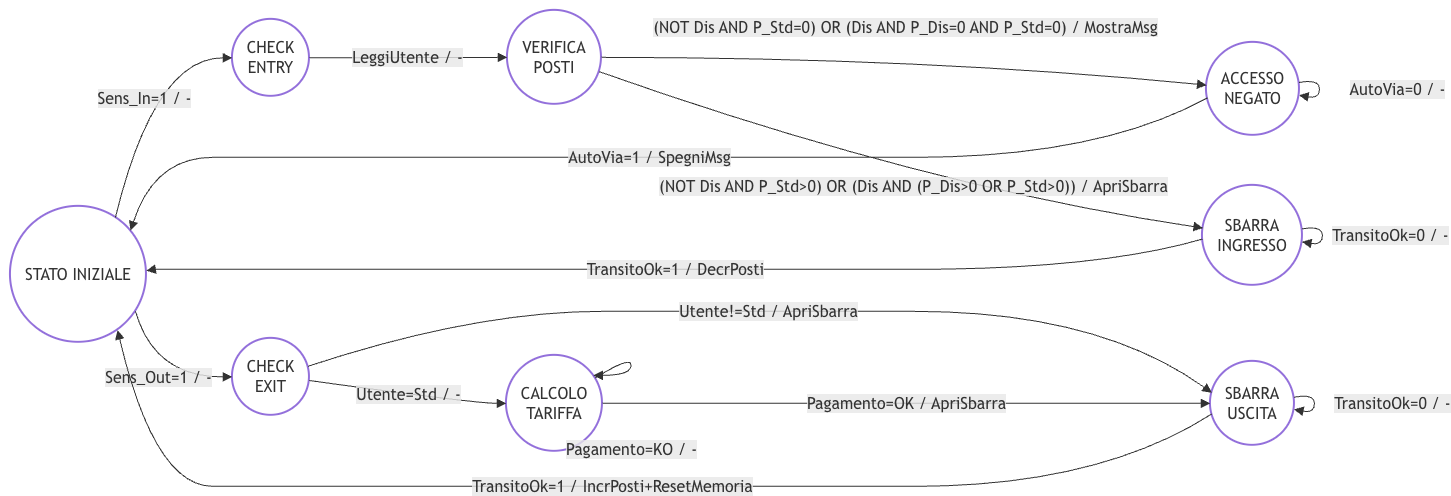
\includegraphics[width=1\linewidth]{images/ASM.drawio.png}
    \caption{Macchina a stati di SmartParking: gli 8 stati e le transizioni, con il ciclo
    di ingresso (CHK\_IN, VER, INGR oppure NEG) e quello di uscita (CHK\_OUT, TARIF, USC).}
    \label{fig:fsm}
\end{figure}



\newpage
\section{Modello Asmeta}

\subsection{Il modello (\texttt{asmeta/src/SmartParking.asm})}

Nel modello ho definito tre domini enumerativi (\texttt{StatoSistema},
\texttt{TipoUtente}, \texttt{TipoPosto}), sei funzioni monitorate (\texttt{sens\_in},
\texttt{sens\_out}, \texttt{transito\_ok}, \texttt{auto\_via}, \texttt{utente\_rilevato},
\texttt{pagamento\_ok}) e quattro funzioni controllate (\texttt{stato},
\texttt{posti\_std}, \texttt{posti\_dis}, \texttt{posto\_assegnato}). A queste ho
aggiunto una funzione derivata n-aria (binaria), \texttt{assegnabile: Prod(TipoUtente,
TipoPosto) $\to$ Boolean}, che raccoglie in un punto solo tutta la politica di
assegnazione: un \texttt{POSTO\_STD} si può dare a chiunque se \texttt{posti\_std > 0},
mentre un \texttt{POSTO\_DIS} è riservato ai disabili e solo se \texttt{posti\_dis > 0}.
Trattandosi di una funzione derivata, viene ricalcolata a ogni stato a partire dalle
funzioni controllate, quindi non occupa memoria.

\begin{lstlisting}[language=Pascal, caption={Funzione derivata assegnabile}]
derived assegnabile: Prod(TipoUtente, TipoPosto) -> Boolean

function assegnabile($u in TipoUtente, $p in TipoPosto) =
    ($p = POSTO_STD and posti_std > 0) or
    ($p = POSTO_DIS and $u = DISABILE and posti_dis > 0)
\end{lstlisting}

Sempre tra le derivate ho aggiunto \texttt{parcheggioPieno}, che uso per far vedere il
costrutto \texttt{forall}: è vera quando, per \emph{ogni} tipo di utente, non è
assegnabile né un posto standard né uno disabile, cioè quando davvero non può più entrare
nessuno. La controllo nello scenario di saturazione \texttt{test\_pieno\_totale.avalla},
dove all'inizio è falsa (c'è ancora posto) e a parcheggio pieno diventa vera.

\begin{lstlisting}[language=Pascal, caption={Funzione derivata parcheggioPieno (uso di forall)}]
function parcheggioPieno =
    (forall $u in TipoUtente with
        (not assegnabile($u, POSTO_STD) and not assegnabile($u, POSTO_DIS)))
\end{lstlisting}

La regola più importante è \texttt{r\_gestione\_VER}, quella che decide a chi assegnare
il posto. Qui ho usato una regola \texttt{let} insieme alla derivata
\texttt{assegnabile}: la regola prova prima con \texttt{POSTO\_DIS} (che è vero solo per
un disabile quando ci sono ancora posti disabili liberi), poi con \texttt{POSTO\_STD}
(il caso di STD e abbonati, ma anche il fallback del disabile quando i posti riservati
sono finiti) e, se non va a buon fine nessuno dei due, nega l'accesso mandando il
sistema in NEG:

\begin{lstlisting}[language=Pascal, caption={Regola r\_gestione\_VER (assegnazione posto, con let e derivata)}]
rule r_gestione_VER =
    let ($u = utente_rilevato) in
        if assegnabile($u, POSTO_DIS) then
            par
                stato := INGR
                posto_assegnato := POSTO_DIS
            endpar
        else
            if assegnabile($u, POSTO_STD) then
                par
                    stato := INGR
                    posto_assegnato := POSTO_STD
                endpar
            else
                stato := NEG
            endif
        endif
    endlet
\end{lstlisting}

Per il model checking ho poi usato una versione semplificata del modello
(\texttt{SmartParking\_MC.asm}). Qui ho lasciato gli if annidati "appiattiti", che si
comportano esattamente allo stesso modo ma rendono più facile la traduzione verso
NuSMV. Sempre per lo stesso motivo, in questo modello i contatori non sono più
\texttt{Integer} ma stanno su un dominio finito \texttt{Posti = \{0..2\}}, dato che
AsmetaSMV non accetta domini infiniti. Ho scelto \texttt{\{0..2\}} e non \texttt{\{0,1\}}
apposta: così le proprietà \texttt{ag(posti\_std <= 1)} e \texttt{ag(posti\_dis <= 1)}
sono verifiche vere e proprie, e non diventano ovvie solo per come è fatto il tipo.

\subsubsection{Simulazione manuale}

Prima di lanciare gli scenari automatici, per prendere un po' di confidenza con il
modello, conviene simulare a mano qualche step con il simulatore di Asmeta.

\screenshot{asmeta_simulator_ingresso_std}{Simulatore -- ingresso STD completo}{%
Aprire \texttt{asmeta/src/SmartParking.asm} in Eclipse e lanciare il simulatore
interattivo. Impostare \texttt{sens\_in=true}, fare Step, poi \texttt{utente\_rilevato=STD}
e proseguire (CHK\_IN$\to$VER, VER$\to$INGR), infine \texttt{transito\_ok=true} e Step.
Lo screenshot deve mostrare la sequenza di stati IDLE$\to$CHK\_IN$\to$VER$\to$INGR$\to$IDLE
con \texttt{posti\_std} che passa da 1 a 0. La colonna State~0 documenta anche lo stato
iniziale (\texttt{stato=IDLE}, sensori a false); si noti che l'animatore mostra le
funzioni solo dal primo stato in cui vengono lette o aggiornate.}

\screenshot{asmeta_simulator_uscita_std}{Simulatore -- uscita STD con pagamento}{%
Proseguendo nella stessa sessione: \texttt{sens\_out=true} $\to$ CHK\_OUT, utente STD
$\to$ TARIF, \texttt{pagamento\_ok=true} $\to$ USC, \texttt{transito\_ok=true} $\to$
IDLE. Lo screenshot deve mostrare il passaggio per TARIF (pagamento) e lo stato finale
con \texttt{posti\_std} tornato a 1 e \texttt{posto\_assegnato = NESSUNO}.}

\subsection{Scenari Avalla}

\begin{longtable}{@{}p{4.2cm}p{8.8cm}@{}}
\toprule
\textbf{Scenario} & \textbf{Obiettivo} \\
\midrule
\endhead
\texttt{test\_abbonato.avalla} & Ciclo completo ABBONATO: ingresso senza pagamento, uscita diretta (salta TARIF). Bug originale corretto: init \texttt{posti\_std} non era 5 ma 1, e lo stato \texttt{PARK} non esiste (è \texttt{IDLE}). \\
\texttt{test\_disabile.avalla} & Ciclo DISABILE: assegnazione POSTO\_DIS, \texttt{posto\_assegnato} resta POSTO\_DIS durante la sosta, azzerato solo in uscita. \\
\texttt{test\_pieno.avalla} & Un utente STD occupa l'unico posto; un secondo STD viene respinto (NEG). \\
\texttt{test\_disabile\_fallback.avalla} & Copre il fallback: un secondo DISABILE, con \texttt{posti\_dis=0}, riceve POSTO\_STD. \\
\texttt{test\_pagamento\_std.avalla} & Ciclo di uscita STD con un pagamento fallito (resta in TARIF) seguito da uno riuscito. \\
\texttt{test\_pieno\_totale.avalla} & Parcheggio completamente saturo (STD + DISABILE), un terzo utente DISABILE viene respinto. \\
\texttt{test\_random\_30steps.avalla} & Scenario \emph{generato automaticamente}: 30 step random eseguiti nel simulatore ed esportati con ``export to avalla'' (saturazione del parcheggio, doppio NEG, ciclo di pagamento TARIF, rientro). \\
\bottomrule
\end{longtable}

\screenshot{asmeta_animator_test_abbonato}{Animazione di test\_abbonato.avalla}{%
Eseguire lo scenario nell'animatore Asmeta. La tabella degli stati deve mostrare la
fase di uscita dell'ABBONATO: CHK\_OUT $\to$ USC \emph{senza passare da TARIF}
(nessun pagamento), con \texttt{posti\_std} che torna a 1 e \texttt{posto\_assegnato}
azzerato a NESSUNO. L'esito dei \texttt{check} (tutti PASSED) è riportato dalla
validazione AsmetaV in console.}

\screenshot{asmeta_animator_test_disabile_fallback}{Animazione di test\_disabile\_fallback.avalla}{%
Stessa procedura per lo scenario di fallback. Deve mostrare i due ingressi DISABILE
consecutivi con l'assegnazione POSTO\_DIS poi POSTO\_STD (fallback), tutti i check verdi.}

\screenshot{asmeta_animator_test_pieno_totale}{Animazione di test\_pieno\_totale.avalla}{%
Stessa procedura per lo scenario di saturazione totale, con il rifiuto (NEG) del
terzo utente e tutti i check verdi.}

\subsection{AsmetaV -- validazione con copertura (Vc)}\label{sec:asmetav-vc}

Gli scenari li ho validati con AsmetaV usando la modalità che calcola anche la
copertura, cioè l'opzione ``Vc'' richiesta dalla consegna. In pratica, per ogni scenario
il validatore non si limita a controllare i \texttt{check}, ma stampa in console anche
quali regole del modello sono state usate (la \emph{rule coverage}). Mettendo insieme i
sei scenari scritti a mano si arriva a coprire tutte le 8 regole di transizione, la main
rule e tutti i rami di \texttt{r\_gestione\_VER}.

A questo punto è interessante confrontare questi scenari con quelli generati a caso. Un
primo export di 15 step random copriva solo 6 regole su 9 (restavano fuori
\texttt{r\_gestione\_NEG}, \texttt{r\_gestione\_TARIF} e \texttt{r\_gestione\_USC});
raddoppiando a 30 step (\texttt{test\_random\_30steps.avalla}) la rule coverage arriva
al 100\%, ma la branch coverage resta comunque incompleta
(\texttt{r\_gestione\_USC} 33\%, \texttt{r\_gestione\_TARIF} 50\%,
\texttt{r\_gestione\_IDLE} 75\%). Il ramo ``pagamento fallito'' di TARIF, per esempio,
non capita quasi mai per caso, e infatti viene coperto solo dallo scenario mirato
\texttt{test\_pagamento\_std}. Insomma, la generazione random è utile come aggiunta, ma
non sostituisce gli scenari scritti a mano sui casi limite.

\screenshot{asmetav_coverage_report}{Report di copertura AsmetaV (Vc)}{%
Tasto destro su ciascun file \texttt{.avalla} $\to$ \textbf{ASMETA $\to$ Validate
scenario and compute coverage} (voce con ``coverage''). Lo screenshot deve mostrare la
console con l'esito dei check (PASSED) e l'elenco delle regole coperte; ripetere per
tutti gli scenari e mostrare (anche cumulativamente) che tutte le regole risultano
coperte.}

\subsection{Model checking (\texttt{asmeta/src/SmartParking\_MC.asm})}

Per il model checking ho scritto 10 CTLSPEC (Tabella~\ref{tab:ctlspec}). Otto me le
aspetto vere e le ho divise in proprietà di sicurezza (safety), di raggiungibilità e di
liveness; le altre due invece le ho messe apposta false, giusto per far vedere che il
model checker, quando una proprietà non regge, tira fuori un controesempio.

\begin{longtable}{@{}p{0.6cm}p{7.3cm}p{2.2cm}p{1.3cm}@{}}
\toprule
\textbf{\#} & \textbf{CTLSPEC} & \textbf{Categoria} & \textbf{Esito} \\
\midrule
\endhead
1  & \texttt{ag(posti\_std >= 0)} & Safety & TRUE \\
2  & \texttt{ag(posti\_dis >= 0)} & Safety & TRUE \\
3  & \texttt{ag((stato=INGR and posto\_assegnato=POSTO\_STD) implies posti\_std>0)} & Safety & TRUE \\
4  & \texttt{ag(posti\_std <= 1)} & Safety & TRUE \\
5  & \texttt{ag(posti\_dis <= 1)} & Safety & TRUE \\
6  & \texttt{ag((stato=INGR and posto\_assegnato=POSTO\_DIS) implies posti\_dis>0)} & Safety & TRUE \\
7  & \texttt{ef(stato = TARIF)} & Raggiungibilità & TRUE \\
8  & \texttt{ag(stato=TARIF implies ef(stato=IDLE))} & Liveness & TRUE \\
9  & \texttt{ag(stato != NEG)} & Falsa (voluta) & FALSE \\
10 & \texttt{ag(stato=TARIF implies af(stato=IDLE))} & Falsa (voluta) & FALSE \\
\bottomrule
\caption{Le 10 CTLSPEC sottoposte ad AsmetaSMV: 8 verificate, 2 volutamente false.}
\label{tab:ctlspec}
\end{longtable}

Le due specifiche false sono interessanti, ognuna a modo suo:

\begin{itemize}
    \item la \#9 dice che ``l'accesso non viene mai negato''. Il controesempio che
    genera NuSMV (9 stati) fa entrare un abbonato che occupa l'unico posto standard;
    poi arriva un secondo veicolo, la verifica non trova posto e il sistema va in NEG,
    e lo fa con il posto disabili ancora libero (\texttt{posti\_dis = 1}). Questa
    traccia dimostra due cose in una volta: che lo stato di rifiuto si può davvero
    raggiungere, e che la riserva funziona, perché il posto disabili non viene dato a
    chi non ne ha diritto;
    \item la \#10 è la versione con \texttt{af} della liveness \#8: chiede che da TARIF
    il sistema torni in IDLE su \emph{ogni} cammino, non solo che esista un cammino che
    ci riporta. È falsa perché nulla vieta all'ambiente di tenere
    \texttt{pagamento\_ok = false} per sempre, cioè un utente che non paga mai, e infatti
    il controesempio è proprio il loop infinito in TARIF. Mettere a confronto la \#8 e la
    \#10 fa vedere bene la differenza tra \texttt{ef} e \texttt{af} in CTL.
\end{itemize}

\screenshot{asmetasmv_ctlspec_results}{Esito delle 10 CTLSPEC in AsmetaSMV}{%
Tasto destro su \texttt{SmartParking\_MC.asm} $\to$ \textbf{Run As $\to$ AsmetaSMV}.
Lo screenshot deve mostrare le 8 specifiche con esito \texttt{is true} e le 2
specifiche volutamente false con esito \texttt{is false}, ciascuna con il proprio
controesempio generato.}

\screenshot{asmetasmv_random_trace}{Esecuzione random-step di verifica manuale}{%
Nella stessa vista AsmetaSMV, usare la funzione di simulazione random (random step)
per generare una traccia di 8-10 stati. Utile per mostrare a voce, all'orale, che il
modello si comporta coerentemente (nessuna transizione viola le regole).}

\subsubsection{Model Advisor (opzionale)}

Il Model Advisor (AsmetaMA) lavora passando per la traduzione in NuSMV, quindi l'ho
lanciato sul modello semplificato \texttt{SmartParking\_MC.asm}: quello principale, con
\texttt{Integer} e funzioni derivate, non è traducibile e dà ``Error Domain Integer not
supported''. L'analisi delle meta-proprietà ha dato questi esiti:

\begin{itemize}
\item \textbf{MP1, MP3, MP4, MP7} non hanno prodotto segnalazioni: nessun aggiornamento
inconsistente, nessuna assegnazione banale, nessuna locazione rimuovibile o mai
aggiornata.
\item \textbf{MP2} (``conditional rule not complete'') scatta su tutte le regole di
transizione, ma si tratta di falsi positivi noti. L'advisor segnala ogni
\texttt{if} privo di \texttt{else}, mentre in ASM l'assenza dell'else è idiomatica e
significa ``nessun aggiornamento'': è proprio il comportamento che serve per i
self-loop della FSM (per esempio \texttt{r\_gestione\_NEG} resta in NEG finché
\texttt{auto\_via} non diventa vero, e \texttt{r\_gestione\_TARIF} resta in TARIF
a pagamento fallito).
\item \textbf{MP5/MP6} (``Domain Posti could be reduced: element \{2\} could be
removed'') non segnala un difetto ma conferma una scelta. Il dominio \texttt{Posti =
\{0..2\}} è stato preso apposta più ampio del necessario, e l'advisor
dimostra che il valore 2 non è mai raggiunto da \texttt{posti\_std}/\texttt{posti\_dis},
cioè la proprietà di capacità \texttt{ag(posti <= 1)} verificata anche dalle
CTLSPEC.
\end{itemize}

\screenshot{model_advisor_output}{Output del Model Advisor (estratto)}{%
Tasto destro su \texttt{SmartParking\_MC.asm} $\to$ \textbf{Model Advisor}. È
sufficiente un estratto rappresentativo della console: l'ideale è MP1 (nessun update
inconsistente), le prime righe di MP2 e le segnalazioni MP5/MP6 sul dominio Posti;
l'elenco completo delle MP2 è riassunto e discusso nel testo.}

\subsubsection{ATGT -- generazione automatica di scenari (opzionale)}

\screenshot{atgt_scenario_list}{Elenco degli scenari generati da ATGT}{%
Tasto destro su \texttt{SmartParking.asm} $\to$ \textbf{Run As $\to$ ATGT}. Mostrare
la lista dei file \texttt{.avalla} generati automaticamente nella cartella di output
(uno screenshot dell'Explorer/Package Explorer di Eclipse con la cartella espansa).}

Gli scenari che ATGT genera (\texttt{asmeta/src/abstractests/testtest*.avalla}) si
possono guardare direttamente nel repository. Il loro ruolo, insieme a quello dello
scenario random da 30 step, l'ho già discusso nel confronto con gli scenari scritti a
mano in \S\ref{sec:asmetav-vc}.

\section{Implementazione Java}

\subsection{Struttura del progetto Maven}

Il progetto Maven (\texttt{java/}) gira su Java 17 e usa Spring Boot con Vaadin 24 per
la UI, JUnit 5 e Mockito per i test e JaCoCo per la copertura. Il cuore del programma sta
nel package \texttt{it.tvsw.smartparking.core}, che contiene:

\begin{itemize}
    \item \texttt{StatoSistema}, \texttt{TipoUtente}, \texttt{TipoPosto}: enum identici ai domini ASM;
    \item \texttt{Parcheggio}: nucleo con contratti JML (Sezione~\ref{sec:jml-ref});
    \item \texttt{SensorInput}: raccoglie i 6 input monitorati di uno step;
    \item \texttt{Display}: interfaccia di notifica (usata per Mockito);
    \item \texttt{SmartParkingFSM}: la macchina a stati, un metodo \texttt{step(SensorInput)} che replica la main rule ASM.
\end{itemize}

\subsection{La macchina a stati}

\begin{lstlisting}[language=Java, caption={step() -- dispatch sullo stato corrente}]
public void step(SensorInput input) {
    switch (stato) {
        case IDLE:     gestisciIdle(input); break;
        case CHK_IN:   gestisciChkIn(); break;
        case VER:      gestisciVer(input); break;
        case NEG:      gestisciNeg(input); break;
        case INGR:     gestisciIngr(input); break;
        case CHK_OUT:  gestisciChkOut(input); break;
        case TARIF:    gestisciTarif(input); break;
        case USC:      gestisciUsc(input); break;
    }
}
\end{lstlisting}

Una nota sul design: nel modello ASM il contatore viene decrementato solo al transito
vero e proprio in INGR, mentre qui la classe \texttt{Parcheggio} decide e decrementa
tutto in un colpo solo, dentro \texttt{assegnaPosto} (che viene chiamato da
\texttt{gestisciVer}). Negli scenari di test del progetto questa differenza non si vede,
e l'ho scelta apposta per tenere il codice più semplice; ne riparlo meglio
nell'osservazione dedicata in Sezione~\ref{sec:analisi-statica}.

\subsection{Interfaccia utente (Vaadin)}

Per la UI ho creato la vista \texttt{MainView}, che mostra lo stato corrente e i posti
ancora liberi. I sensori li ho simulati con dei bottoni: ``Arriva auto
STD/DISABILE/ABBONATO'', ``Transito'', ``Pagamento'', ``Auto va via'' e ``Auto in
uscita''. In pratica cliccando i bottoni si fa avanzare la macchina a stati come se
arrivassero gli input dai sensori veri.

\screenshot{vaadin_ui_idle}{UI Vaadin -- stato iniziale}{%
Lanciare \texttt{cd java \&\& mvn spring-boot:run}, aprire
\url{http://localhost:8080}. Screenshot della pagina appena caricata: stato IDLE,
posti standard liberi = 1, posti disabili liberi = 1.}

\screenshot{vaadin_ui_ingresso_std}{UI Vaadin -- dopo un ingresso STD}{%
Cliccare ``Arriva auto STD'' poi ``Transito''. Screenshot che mostra lo stato
aggiornato (IDLE) e posti standard liberi = 0.}

\screenshot{vaadin_ui_neg}{UI Vaadin -- accesso negato a parcheggio pieno}{%
Con il parcheggio pieno (posti standard e disabili a 0), cliccare di nuovo un
bottone ``Arriva auto...''. Screenshot che mostra il messaggio ``Accesso negato''.}

\screenshot{vaadin_ui_tarif}{UI Vaadin -- attesa pagamento}{%
Dopo un ingresso STD e un ``Transito'', cliccare ``Auto in uscita'': lo stato deve
mostrare TARIF (in attesa di pagamento) prima di cliccare ``Pagamento''.}

\subsection{Test end-to-end con Selenium}

La UI l'ho controllata anche con un test end-to-end fatto in Selenium
(\texttt{UISeleniumTest}). L'ho taggato ``ui'' e l'ho escluso dalla build normale, perché
per girare ha bisogno dell'applicazione già avviata e di Chrome. Quello che fa è aprire
la pagina con ChromeDriver in modalità headless, aspettare che Vaadin finisca di
renderizzare lato client (con \texttt{WebDriverWait}), cliccare ``Arriva auto STD'' e
controllare che lo stato mostrato diventi INGR o NEG. Per lanciarlo basta
\texttt{mvn test -Dtest.groups=ui -Dtest.excludedGroups=}, oppure eseguirlo da Eclipse
come un normale test JUnit.

\screenshot{selenium_test_green}{Test Selenium end-to-end superato}{%
Vista JUnit di Eclipse (o terminale Maven) con \texttt{UISeleniumTest} verde,
eseguito con l'applicazione attiva su localhost:8080.}

\section{Testing Java}
\label{sec:testing}

\subsection{Struttura dei test}

Ho diviso i test in più classi, una per ogni aspetto che volevo coprire, così è più
facile capire cosa controlla cosa. Nella tabella qui sotto ho messo l'elenco con,
accanto, quello che ciascuna classe va a verificare.

\begin{longtable}{@{}p{4.3cm}p{8.7cm}@{}}
\toprule
\textbf{Classe} & \textbf{Copre} \\
\midrule
\endhead
\texttt{ParcheggioTest} & Costruttori, precondizioni violate, tutti i rami di \texttt{assegnaPosto}/\texttt{liberaPosto}, test parametrico CSV. \\
\texttt{SmartParkingFSMTest} & Tutti gli 8 stati e le transizioni, fallback disabile, parcheggio pieno, self-loop NEG/INGR/TARIF. \\
\texttt{McdcVerificaTest} & Copertura MC/DC delle due decisioni composte di \texttt{assegnaPosto} (Tabella~\ref{tab:mcdc1} e~\ref{tab:mcdc2}). \\
\texttt{DisplayMockTest} & Notifiche a \texttt{Display} verificate con Mockito. \\
\texttt{ScenarioAvallaTest} & Traduzione fedele di \texttt{test\_pieno.avalla} in JUnit (Model Based Testing). \\
\texttt{CombinatorialTest} & Tabella pairwise a 6 righe (Tabella~\ref{tab:pairwise}). \\
\texttt{UISeleniumTest} & Smoke test della UI (tag \texttt{ui}, escluso dalla build standard). \\
\bottomrule
\end{longtable}

\subsection{MC/DC}

Dentro \texttt{assegnaPosto} ci sono due decisioni composte, cioè con più condizioni
messe in and/or, e per queste ho voluto una copertura MC/DC vera e propria: per ogni
condizione serve una coppia di casi di test in cui, cambiando solo quella condizione,
cambia anche il risultato della decisione. Vediamole una alla volta.

La prima decisione è quella del ramo STD/ABBONATO: $D_1 = (\text{utente}{=}\text{STD}
\lor \text{utente}{=}\text{ABBONATO}) \land \text{postiStd}{>}0$.

\begin{longtable}{@{}p{1cm}p{0.6cm}p{0.6cm}p{0.6cm}p{0.6cm}p{2.6cm}p{5.5cm}@{}}
\toprule
Caso & A & B & C & $D_1$ & Esito & Coppia indipendente \\
\midrule
\endhead
TC1 & T & F & T & T & POSTO\_STD & base \\
TC2 & T & F & F & F & NESSUNO & isola C (vs TC1) \\
TC3 & F & F & T & F & POSTO\_DIS & isola A (vs TC1) \\
TC4 & F & T & T & T & POSTO\_STD & isola B (vs TC3) \\
\bottomrule
\caption{MC/DC -- Decisione 1.}
\label{tab:mcdc1}
\end{longtable}

La seconda decisione è quella del ramo DISABILE, cioè il fallback, con
$C_1{=}\text{postiDis}{>}0$ e $C_2{=}\text{postiStd}{>}0$.

\begin{longtable}{@{}p{1cm}p{1cm}p{1cm}p{2.6cm}p{6.5cm}@{}}
\toprule
Caso & $C_1$ & $C_2$ & Esito & Coppia indipendente \\
\midrule
\endhead
TC5 & T & --- & POSTO\_DIS & base \\
TC6 & F & T & POSTO\_STD & isola $C_1$ (vs TC5) \\
TC7 & F & F & NESSUNO & isola $C_2$ (vs TC6) \\
\bottomrule
\caption{MC/DC -- Decisione 2.}
\label{tab:mcdc2}
\end{longtable}

\subsection{Combinatorial testing (pairwise)}

L'assegnazione del posto dipende da tre parametri: il tipo di utente
(\texttt{tipoUtente} $\in$ \{STD, DISABILE, ABBONATO\}), i posti standard liberi
(\texttt{postiStd} $\in \{0, 1\}$) e quelli disabili liberi (\texttt{postiDis}
$\in \{0, 1\}$). Provare tutte le combinazioni sarebbe possibile ma inutile: mi basta
coprire tutte le \emph{coppie} di valori, ed è quello che fa la tabella pairwise qui
sotto, che con sole 6 righe le copre tutte.

\begin{longtable}{@{}p{0.6cm}p{2cm}p{1.6cm}p{1.6cm}p{3.5cm}@{}}
\toprule
\# & tipoUtente & postiStd & postiDis & Esito atteso \\
\midrule
\endhead
1 & STD      & 0 & 0 & NESSUNO \\
2 & STD      & 1 & 1 & POSTO\_STD \\
3 & DISABILE & 0 & 1 & POSTO\_DIS \\
4 & DISABILE & 1 & 0 & POSTO\_STD (fallback) \\
5 & ABBONATO & 0 & 1 & NESSUNO \\
6 & ABBONATO & 1 & 0 & POSTO\_STD \\
\bottomrule
\caption{Tabella pairwise (copre tutte le coppie dei 3 parametri).}
\label{tab:pairwise}
\end{longtable}

\subsection{Mockito}

La FSM, a ogni cambio di stato, manda un messaggio a un oggetto \texttt{Display}. Per
controllare che questi messaggi partano davvero, senza dover tirare in ballo la UI vera,
ho usato Mockito: creo un finto \texttt{Display} e poi con \texttt{verify} controllo che
il metodo \texttt{mostra} venga chiamato con il testo giusto. Nell'esempio qui sotto
riempio il parcheggio e verifico che, al terzo ingresso, il display riceva davvero
``Accesso negato''.

\begin{lstlisting}[language=Java, caption={Verifica delle notifiche con Mockito}]
@Test
void notificaAccessoNegatoQuandoParcheggioPieno() {
    SmartParkingFSM fsm = new SmartParkingFSM(new Parcheggio(0, 0), display);
    fsm.step(SensorInput.sensIn());
    fsm.step(SensorInput.utente(TipoUtente.STD));
    fsm.step(SensorInput.utente(TipoUtente.STD));
    verify(display).mostra("Accesso negato");
}
\end{lstlisting}

\subsection{Model Based Testing}

L'idea del model based testing è prendere uno scenario già scritto sul modello astratto
e tradurlo in un test sul codice vero. Ho preso lo scenario \texttt{test\_pieno.avalla} e
l'ho riportato passo passo in \texttt{ScenarioAvallaTest}: ogni blocco
\texttt{set}/\texttt{step}/\texttt{check} dell'avalla diventa la corrispondente riga
JUnit, e ho lasciato un commento accanto a ciascuna per richiamare la riga originale
dello scenario.

\subsection{Esecuzione e copertura}

\screenshot{junit_run_all_green}{Esecuzione di tutta la suite JUnit}{%
In Eclipse (o IntelliJ), tasto destro sulla cartella \texttt{src/test/java} $\to$
\textbf{Run As $\to$ JUnit Test}, oppure da terminale \texttt{mvn test}. Screenshot
della vista JUnit con tutti i test verdi e il conteggio totale (es. ``Runs: N/N,
Errors: 0, Failures: 0'').}

La copertura l'ho misurata con JaCoCo, lanciando \texttt{mvn verify} e guardando il
report in \texttt{target/site/jacoco/index.html}. Dal conteggio ho tolto la UI Vaadin
(che testo end-to-end con Selenium e che JaCoCo non riesce a misurare) e la classe di
avvio di Spring Boot, che sono solo 3 righe di boilerplate; l'esclusione è scritta nel
\texttt{pom.xml}. Alla prima misurazione il package \texttt{core} stava al 98\% di
instruction e al 95\% di branch. La classe \texttt{Parcheggio} era già al 100\%/100\%
(coerente con la verifica ESC dei contratti, \S\ref{sec:jml-ref}), mentre in
\texttt{SmartParkingFSM} restavano scoperti 3 branch: il self-loop di
\texttt{gestisciUsc} (\texttt{transito\_ok} falso in USC), il ramo
\texttt{display == null} di \texttt{cambiaStato} e il \texttt{default} dello switch di
\texttt{step}. I primi due erano veri buchi di test, che ho chiuso aggiungendo due
test mirati (\texttt{uscRestaInUscFinoAlTransito}, \texttt{fsmFunzionaSenzaDisplay}).
Il terzo invece non è raggiungibile: lo switch gestisce tutti e 8 i valori dell'enum
\texttt{StatoSistema}, per cui il \texttt{default} (difensivo, lancia
\texttt{IllegalStateException}) non può mai essere eseguito. È l'analogo Java dei rami
infattibili già osservati con AsmetaV sul modello (\S\ref{sec:asmetav-vc}). Dopo aver
aggiunto i due test, quel \texttt{default} resta l'unico branch non coperto del
package.

\screenshot{jacoco_coverage_report}{Report JaCoCo -- totale (solo package core)}{%
Pagina principale del report (stato finale, dopo l'aggiunta dei due test mirati):
98\% instruction / 98\% branch coverage; l'unico elemento non coperto e' 1 branch su
61 (il \texttt{default} difensivo dello switch, strutturalmente irraggiungibile).}

\screenshot{jacoco_detail_parcheggio}{Report JaCoCo -- dettaglio per classe del package core}{%
Vista del package \texttt{it.tvsw.smartparking.core}: \texttt{Parcheggio} 100\%/100\%,
enum e \texttt{SensorInput} 100\%, \texttt{SmartParkingFSM} 96\%/96\%.}

\screenshot{jacoco_detail_fsm}{Report JaCoCo -- dettaglio per metodo di SmartParkingFSM}{%
Vista per metodo di \texttt{SmartParkingFSM}: tutti i metodi al 100\% tranne
\texttt{step()}, il cui unico branch non coperto è il \texttt{default} difensivo
dello switch, strutturalmente irraggiungibile (discusso nel testo).}

\section{JML e verifica statica (ESC)}
\label{sec:jml-ref}

Per la parte di design by contract ho annotato con JML una classe sola,
\texttt{Parcheggio}. È il nucleo del dominio: tiene i due contatori dei posti liberi e
gestisce l'assegnazione e il rilascio, cioè fa quello che nel modello ASM fanno le regole
\texttt{r\_gestione\_VER}, \texttt{r\_gestione\_INGR} e \texttt{r\_gestione\_USC}.

L'ho tenuta piccola apposta e senza dipendenze da niente: dentro ci sono solo
\texttt{int} ed enum. Il motivo è pratico, cioè che così OpenJML riesce a dimostrarla
tutta, mentre su una classe che si tira dietro mezzo Spring non ci sarei mai arrivato.
Tutto il resto del sistema (la FSM, la UI, il display, i sensori) è Java normale senza
annotazioni, come chiedeva la consegna.

Una cosa che ho scoperto sbattendoci contro: i campi \texttt{postiStd} e
\texttt{postiDis} li ho dovuti dichiarare \texttt{private /*@ spec\_public @*/}. Le
clausole di specifica public, come le invarianti e le postcondizioni, possono nominare
solo roba visibile a livello public, e se lascio i campi semplicemente private OpenJML si
ferma con un errore di visibilità. Con \texttt{spec\_public} restano private per il
codice ma diventano visibili alla specifica.

\subsection{Invarianti}

Le invarianti sono due e devono valere sempre, da dopo il costruttore in poi:

\begin{itemize}
\item i posti standard liberi stanno sempre tra 0 e \texttt{MAX\_STD};
\item i posti disabili liberi stanno sempre tra 0 e \texttt{MAX\_DIS}.
\end{itemize}

\begin{lstlisting}[style=terminal, caption={Invarianti di classe}]
//@ public invariant 0 <= postiStd && postiStd <= MAX_STD;
private /*@ spec_public @*/ int postiStd;

//@ public invariant 0 <= postiDis && postiDis <= MAX_DIS;
private /*@ spec_public @*/ int postiDis;
\end{lstlisting}

Sono le stesse identiche proprietà che avevo già verificato con il model checking sul
modello, cioè \texttt{ag(posti >= 0)} e \texttt{ag(posti <= 1)}. Le ho scritte apposta
uguali: così la stessa cosa finisce garantita a tre livelli diversi, nel modello con il
model checker, nel codice con il contratto, e ancora nei test con JaCoCo.

\subsection{Costruttori}

I costruttori sono due. Quello di default garantisce lo stato iniziale del modello ASM,
cioè tutti i posti liberi. Quello con i parametri lo uso nei test, quando mi serve
partire da una configurazione qualunque, e chiede che i valori passati siano già dentro i
limiti dell'invariante.

\begin{lstlisting}[style=terminal, caption={Contratti dei costruttori}]
//@ ensures postiStd == MAX_STD && postiDis == MAX_DIS;
public Parcheggio() { ... }

//@ requires 0 <= postiStdIniziali && postiStdIniziali <= MAX_STD;
//@ requires 0 <= postiDisIniziali && postiDisIniziali <= MAX_DIS;
//@ ensures postiStd == postiStdIniziali && postiDis == postiDisIniziali;
public Parcheggio(int postiStdIniziali, int postiDisIniziali) { ... }
\end{lstlisting}

Il \texttt{requires} del secondo costruttore dice cosa deve garantire chi chiama, ma non
protegge a runtime: se qualcuno passa un valore fuori range senza aver fatto la verifica
statica, il contratto non lo ferma. Per questo dentro ho messo anche un controllo
esplicito che lancia \texttt{IllegalArgumentException}, e quel comportamento lo provo in
\texttt{ParcheggioTest} con \texttt{assertThrows}.

\subsection{Metodo \texttt{assegnaPosto}}

Questo è quello con il contratto più lungo, perché deve dire tutto quello che fa
\texttt{r\_gestione\_VER}. Le postcondizioni sono due, una per ramo.

Per STD e ABBONATO ci sono due esiti possibili: o c'era un posto standard libero, e
allora torna \texttt{POSTO\_STD} con il contatore sceso di 1, oppure non c'era e torna
\texttt{NESSUNO} senza toccare niente.

Per il DISABILE gli esiti sono tre, perché in mezzo c'è il fallback: posto disabile se
disponibile, altrimenti posto standard se disponibile, altrimenti \texttt{NESSUNO}.

\begin{lstlisting}[style=terminal, caption={Contratto di assegnaPosto}]
//@ requires utente != null;
//@ ensures (utente == TipoUtente.STD || utente == TipoUtente.ABBONATO) ==>
//@     ((\old(postiStd) > 0 && \result == TipoPosto.POSTO_STD
//@       && postiStd == \old(postiStd) - 1 && postiDis == \old(postiDis))
//@      || (\old(postiStd) == 0 && \result == TipoPosto.NESSUNO
//@       && postiStd == \old(postiStd) && postiDis == \old(postiDis)));
//@ ensures utente == TipoUtente.DISABILE ==>
//@     ((\old(postiDis) > 0 && \result == TipoPosto.POSTO_DIS
//@       && postiDis == \old(postiDis) - 1 && postiStd == \old(postiStd))
//@      || (\old(postiDis) == 0 && \old(postiStd) > 0
//@       && \result == TipoPosto.POSTO_STD
//@       && postiStd == \old(postiStd) - 1 && postiDis == \old(postiDis))
//@      || (\old(postiDis) == 0 && \old(postiStd) == 0
//@       && \result == TipoPosto.NESSUNO
//@       && postiStd == \old(postiStd) && postiDis == \old(postiDis)));
public TipoPosto assegnaPosto(TipoUtente utente) { ... }
\end{lstlisting}

Il \texttt{\textbackslash old} serve per parlare del valore che il contatore aveva prima
della chiamata, altrimenti non potrei dire ``è sceso di uno''.

Una cosa che all'inizio non avevo messo: in ogni esito ho anche scritto che l'\emph{altro}
contatore resta com'era. Senza quel pezzo il contratto sarebbe stato sottospecificato,
cioè un'implementazione che assegna il posto giusto ma nel frattempo tocca anche l'altro
contatore lo rispetterebbe lo stesso.

\subsection{Metodo \texttt{liberaPosto}}

Questo corrisponde al rilascio del posto in \texttt{r\_gestione\_USC}. Chiede che il
posto non sia null e che il contatore corrispondente non sia già al massimo, e garantisce
che venga incrementato di 1 solo quello giusto. Con \texttt{NESSUNO} non fa niente e lo
stato resta identico.

\begin{lstlisting}[style=terminal, caption={Contratto di liberaPosto}]
//@ requires posto != null;
//@ requires posto == TipoPosto.POSTO_STD ==> postiStd < MAX_STD;
//@ requires posto == TipoPosto.POSTO_DIS ==> postiDis < MAX_DIS;
//@ ensures posto == TipoPosto.POSTO_STD ==>
//@     postiStd == \old(postiStd) + 1 && postiDis == \old(postiDis);
//@ ensures posto == TipoPosto.POSTO_DIS ==>
//@     postiDis == \old(postiDis) + 1 && postiStd == \old(postiStd);
//@ ensures posto == TipoPosto.NESSUNO ==>
//@     postiStd == \old(postiStd) && postiDis == \old(postiDis);
public void liberaPosto(TipoPosto posto) { ... }
\end{lstlisting}

Quel secondo e terzo \texttt{requires} non c'erano nella prima versione e sono il motivo
per cui la prova non chiudeva: ne parlo tra poco.

\subsection{Metodi getter}

I due getter li ho annotati \texttt{/*@ pure @*/}, che vuol dire senza effetti
collaterali. Serve perché un metodo non puro dentro una clausola JML non si può usare. La
postcondizione dice solo che restituiscono il campo, niente di più.

\begin{lstlisting}[style=terminal, caption={Getter puri}]
//@ ensures \result == postiStd;
public /*@ pure @*/ int getPostiStd() { ... }

//@ ensures \result == postiDis;
public /*@ pure @*/ int getPostiDis() { ... }
\end{lstlisting}

\subsection{Verifica dei contratti con OpenJML (ESC)}

Scritti i contratti, li ho verificati con OpenJML (release 21.0.27, build nativa per
macOS arm64) in modalità \texttt{--esc}. Quello che fa il tool è tradurre codice e
contratti in formule logiche e passarle al solver Z3, che deve dimostrare che
\emph{qualunque} esecuzione rispetta postcondizioni e invarianti. È una cosa diversa dai
test: i test provano alcuni casi, qui invece o si dimostra per tutti o non si dimostra.

Il comando, dalla root del progetto, è questo:

\begin{lstlisting}[style=terminal, caption={Comando di verifica ESC}]
$ openjml --esc --progress \
    -cp java/src/main/java \
    java/src/main/java/it/tvsw/smartparking/core/Parcheggio.java
\end{lstlisting}

\subsubsection*{Un contratto che all'inizio non chiudeva}

Arrivare a ``tutti Verified'' non è stato immediato, e il caso di \texttt{liberaPosto}
secondo me è quello che spiega meglio come funziona la cosa.

La prima versione che avevo scritto era questa, con la postcondizione che descrive
l'incremento ma senza il \texttt{requires} sulla capacità:

\begin{lstlisting}[style=terminal, caption={Prima versione di liberaPosto (senza il requires di capacità)}]
//@ requires posto != null;
//@ ensures posto == TipoPosto.POSTO_STD ==>
//@     postiStd == \old(postiStd) + 1 && postiDis == \old(postiDis);
public void liberaPosto(TipoPosto posto) { ... }
\end{lstlisting}

Il solver, non avendo nessun vincolo sul valore di partenza, prova anche il caso
\texttt{postiStd == MAX\_STD}. Lì \texttt{postiStd + 1} fa \texttt{MAX\_STD + 1}, che
viola l'invariante di classe. Quindi non riesce a ristabilire l'invariante all'uscita del
metodo e mi risponde così:

\begin{lstlisting}[style=terminal, caption={Errore ESC sulla prima versione}]
Parcheggio.java:.. warning: The prover cannot establish an assertion
   (InvariantExit) in method liberaPosto
   postiStd == \old(postiStd) + 1 ...
   Associated declaration: invariant 0 <= postiStd && postiStd <= MAX_STD
\end{lstlisting}

La soluzione è rafforzare la precondizione, in modo che sia chi chiama a garantire che
c'è spazio per incrementare:

\begin{lstlisting}[style=terminal, caption={Versione corretta: il requires di capacità chiude la prova}]
//@ requires posto == TipoPosto.POSTO_STD ==> postiStd < MAX_STD;
//@ requires posto == TipoPosto.POSTO_DIS ==> postiDis < MAX_DIS;
\end{lstlisting}

Con \texttt{postiStd < MAX\_STD} assunto all'ingresso, dopo l'incremento vale
\texttt{postiStd <= MAX\_STD}, l'invariante regge e il metodo passa a Verified.

Il senso della cosa, secondo me, è questo: ogni volta che c'è un'operazione aritmetica
bisogna aver vincolato prima tutto quello che ci entra, con un \texttt{requires} o con
un'invariante. \texttt{Parcheggio} chiude tutto perché ha due soli interi e tutti e due
sono limitati; su un nucleo con array o contatori liberi la stessa cosa diventa molto più
difficile. L'altro ostacolo che ho incontrato era di tutt'altro tipo, cioè la visibilità
dei campi private, e l'ho risolto con \texttt{spec\_public} come ho detto all'inizio.

\screenshot{openjml_esc_output}{Output di \texttt{openjml --esc}: tutti i metodi Verified}{%
Esito Verified per tutti e sei i metodi di Parcheggio, senza righe ``cannot be proved''.}

Alla fine tutti e sei i metodi (i due costruttori, \texttt{assegnaPosto},
\texttt{liberaPosto} e i due getter) risultano Verified.

\section{Ispezione del codice e analisi statica}
\label{sec:analisi-statica}

Questa parte l'ho affrontata in tre passaggi diversi, perché ognuno trova cose che gli
altri due si perdono: prima l'ispezione manuale con la checklist vista a lezione, poi
una seconda lettura fatta fare a un LLM, e infine l'analisi automatica con SpotBugs.

\subsection{Ispezione con la checklist}
\label{sec:checklist}

La prima passata l'ho fatta con la checklist di code inspection del corso, andando in
ordine sulle nove categorie. Sotto riporto per ognuna cosa è venuto fuori. Alcune voci
sul mio codice non si applicano proprio, e lo dico invece di spuntarle a vuoto.

\paragraph{1. Specification / Design.}
La funzionalità descritta nei requisiti c'è tutta: ogni requisito da RF1 a RF14 ha il
suo corrispettivo in \texttt{SmartParkingFSM} o in \texttt{Parcheggio}. Di funzionalità
in più rispetto alla specifica non ne ho trovate: i due metodi che sembravano candidati,
\texttt{SensorInput.nessunEvento()} e il costruttore \texttt{SmartParkingFSM(Display)},
sono entrambi usati dai test, il primo per provare i self-loop (uno step senza nessun
sensore attivo) e il secondo per costruire la FSM con il parcheggio di default.

\paragraph{2. Initialization and Declarations.}
Tutti i campi sono inizializzati nel costruttore, e quelli che non cambiano mai
(\texttt{parcheggio}, \texttt{display}, tutti i campi di \texttt{SensorInput}) sono
\texttt{final}. I tipi sono quelli giusti: gli stati e i tipi di utente sono enum e non
interi o stringhe, quindi un valore fuori dominio non è nemmeno rappresentabile. Tutti i
campi sono \texttt{private}, e \texttt{SensorInput} è dichiarata \texttt{final} e
immutabile.

\paragraph{3. Method Calls.}
Qui è uscita la segnalazione più concreta di tutta la checklist, e non l'aveva vista
nessun altro controllo. Ci sono due firme con \textbf{parametri adiacenti dello stesso
tipo}:

\begin{lstlisting}[language=Java, caption={Firme con parametri adiacenti dello stesso tipo}]
public Parcheggio(int postiStdIniziali, int postiDisIniziali)

public SensorInput(boolean sensIn, boolean sensOut, boolean transitoOk,
                   boolean autoVia, TipoUtente utenteRilevato, boolean pagamentoOk)
\end{lstlisting}

Se in una chiamata scambio i due \texttt{int}, o due dei quattro \texttt{boolean}, il
codice compila senza un fiato e il comportamento cambia. È esattamente il tipo di errore
che la categoria 3 della checklist va a cercare, e che né il compilatore né i contratti
JML possono intercettare, perché a livello di tipi la chiamata è corretta.

Su \texttt{SensorInput} il problema in pratica non si presenta, perché il costruttore non
lo chiama mai nessuno direttamente: si passa sempre dai metodi statici
(\texttt{sensIn()}, \texttt{transito()}, \texttt{pagamento(esito)}\dots), che hanno zero
o un parametro e un nome che dice cosa fanno. È una protezione che avevo messo per
comodità di scrittura dei test, e che a posteriori risolve anche questo.

Su \texttt{Parcheggio(int, int)} invece il rischio resta. L'ho lasciato così perché quel
costruttore lo usano solo i test, dove i valori sono scritti in chiaro riga per riga e un
eventuale scambio farebbe fallire subito l'assert. In un sistema vero la soluzione
sarebbe un tipo dedicato per i due contatori, o un costruttore con \emph{builder}.

\paragraph{4. Arrays.}
Non applicabile: nel progetto non c'è nessun array né nessuna collezione. Lo stato è
tenuto in due interi e in due enum. Di conseguenza non ci sono errori di indice
off-by-one né rischi di sforare i limiti.

\paragraph{5. Object Comparison.}
Tutti i confronti tra enum sono fatti con \texttt{==}, che per gli enum Java è corretto e
anzi preferibile a \texttt{equals}. Stringhe da confrontare non ce ne sono: le uniche che
compaiono sono i messaggi passati al display, che vengono solo scritti, mai testati per
uguaglianza nel codice di produzione.

\paragraph{6. Output Format.}
I messaggi del display sono coerenti e senza errori di battitura. Due osservazioni
minori. La prima è che alcune stringhe sono ripetute in più punti (``Sistema pronto''
compare tre volte, una per ogni ritorno in IDLE): andrebbero in costanti, ma su quattro
messaggi in croce ho lasciato stare. La seconda è che ``Sbarra aperta'' e ``Sbarra di
uscita aperta'' sembrano un'incoerenza e invece sono volute, perché distinguono le due
sbarre.

\paragraph{7. Computation, Comparisons and Assignments.}
Divisioni non ce ne sono, quindi il problema del denominatore a zero non si pone.
L'aritmetica è solo somma e sottrazione di 1 sui due contatori, e non può andare in
overflow perché i contatori sono limitati tra 0 e la capacità massima, cosa garantita in
tre modi diversi: dall'invariante JML, dai controlli a runtime in \texttt{liberaPosto} e
dalle CTLSPEC sul modello. Vale la pena dirlo perché l'overflow è il classico punto in
cui la verifica ESC si inceppa, e qui non succede proprio grazie a quei vincoli.

\paragraph{8. Exceptions.}
Nel progetto non c'è nemmeno un \texttt{try/catch}. È una scelta: le uniche eccezioni
lanciate (\texttt{IllegalArgumentException} e \texttt{IllegalStateException}) segnalano
errori di programmazione, non condizioni che possono capitare a runtime, quindi devono
propagare e non essere nascoste. Un punto di attenzione però c'è: nei gestori dei bottoni
della UI Vaadin non c'è nessuna gestione, quindi un'eccezione lì diventerebbe una pagina
di errore del framework. Per un prototipo va bene, in una versione vera ci vorrebbe un
messaggio all'utente.

\paragraph{9. Flow of Control.}
Lo \texttt{switch} di \texttt{step} ha tutti i \texttt{case} chiusi da \texttt{break} e
un ramo \texttt{default} che lancia eccezione, quindi niente fall-through accidentale.
Il problema del \emph{dangling else} non si presenta: l'unico punto con due condizioni in
fila, \texttt{gestisciIdle}, usa un \texttt{if/else if} esplicito. Infine, nel package
\texttt{core} non c'è \textbf{nessun ciclo}: la FSM avanza di un passo per chiamata e
l'iterazione, se serve, la fa il chiamante. Questo spiega anche perché nella parte JML
(Sezione~\ref{sec:jml-ref}) non compare nessuna \texttt{loop\_invariant}: non essendoci
loop, non c'è niente da invariantizzare.

\subsection{Seconda lettura con un LLM}
\label{sec:llm-review}

La consegna chiedeva di fare l'ispezione ``con chatgpt o LLM in generale'', quindi dopo
la checklist ho usato ChatGPT come se fosse un collega a cui far dare una seconda
occhiata al codice. Gli ho passato tutto il sorgente dei package \texttt{core} e
\texttt{ui} e gli ho chiesto di leggerlo cercando nomi poco chiari, casi limite non
gestiti, possibili \texttt{NullPointerException} e punti in cui il codice si allontana
dal modello ASM.

Le cose che sono uscite non le ho prese per buone così com'erano: le ho valutate una per
una, decidendo di volta in volta se correggerle, mitigarle o lasciarle stare spiegando
perché. L'LLM ha segnalato i punti su cui ragionare, le decisioni le ho prese io.

\begin{enumerate}
    \item \textbf{Manca il controllo di null su \texttt{utenteRilevato} in CHK\_OUT}: il
    confronto restituisce false senza dire niente, e il sistema va in USC come se
    l'utente non fosse STD. L'ho lasciata così per restare fedele all'ASM, dove il
    dominio \texttt{TipoUtente} non prevede l'assenza del dato; in più tutti i punti che
    chiamano quel metodo impostano sempre l'utente.

    \item \textbf{\texttt{TipoPosto.NESSUNO} vuol dire due cose diverse}: in
    \texttt{assegnaPosto} significa ``non c'è posto'', in \texttt{liberaPosto} significa
    ``non fare niente''. Chiarito nel Javadoc, invece di inventare un tipo separato che
    avrebbe appesantito una classe che doveva restare semplice.

    \item \textbf{\texttt{liberaPosto} lancia eccezione se il contatore è già al
    massimo}. Questa l'ho tenuta apposta: preferisco un crash che si vede subito a un
    contatore che va oltre la capacità senza dire niente, violando l'invariante. Il caso
    è comunque coperto da un test.

    \item \textbf{Il decremento avviene in un momento diverso rispetto all'ASM}: qui
    \texttt{assegnaPosto} decide e scala insieme, nell'ASM si scala al transito. Negli
    scenari di test la differenza non si vede, quindi resta la versione più semplice,
    scritta nel Javadoc della classe.

    \item \textbf{Non c'è thread-safety}. Va bene così, perché c'è un varco solo pilotato
    da una FSM sequenziale, esattamente come nel modello. Resta segnata come limite se un
    giorno si volessero gestire più varchi.

    \item \textbf{\texttt{posto\_assegnato} è una memoria da un posto solo, e il difetto
    c'è anche nel modello ASM}. Questa è l'osservazione più importante di tutte. Sia la
    FSM Java sia l'ASM si ricordano un solo posto assegnato, ma nel parcheggio ci stanno
    due veicoli, uno standard e uno disabile. Se entra uno STD, poi entra un DISABILE che
    sovrascrive lo slot, e poi esce il primo, viene rilasciato il posto sbagliato e i
    contatori si sballano.

    Il punto è che l'implementazione è fedele alla specifica: è la specifica stessa che
    dà per scontato di tracciare un veicolo alla volta, senza mai associare un veicolo al
    suo posto. Per sistemarlo servirebbe una mappa veicolo$\to$posto sia nell'ASM sia in
    Java. L'ho lasciato e documentato come limite noto, perché mi sembra l'esempio più
    utile di tutto il progetto: è un difetto che il testing di conformità non può
    trovare, visto che il codice fa esattamente quello che dice il modello, e che salta
    fuori solo leggendo il codice con occhio critico.

    \item \textbf{I bottoni della UI sono sempre attivi}: \texttt{MainView} non li
    disabilita in base allo stato, quindi si può cliccare ``Pagamento'' mentre siamo in
    IDLE. Non succede niente di male perché quegli step finiscono assorbiti dai
    self-loop della FSM, cioè proprio dagli \texttt{if} senza \texttt{else} che il Model
    Advisor segnalava come MP2 (\S\ref{sec:asmetav-vc}). Per un prototipo va bene; in una
    versione vera si metterebbe un \texttt{setEnabled} legato allo stato.
\end{enumerate}

\subsection{Bilancio}

Fra checklist e LLM sono uscite otto osservazioni. Nessun bug vero da correggere nel
codice, e in due casi mi è bastato chiarire le cose nel Javadoc.

Quello che mi ha colpito è che i due metodi hanno trovato cose diverse. La checklist,
proprio perché è meccanica e va per categorie, mi ha fatto guardare le \emph{firme} dei
metodi, che leggendo il codice per capire cosa fa non guardi mai, e da lì è saltato fuori
il problema dei parametri adiacenti dello stesso tipo. L'LLM, che invece ragiona sul
significato, ha trovato il difetto della memoria a slot singolo, che una checklist non
avrebbe mai potuto vedere perché non è una violazione di nessuna regola: è il modello a
essere incompleto.

E quel difetto, il punto 6, è la cosa più utile emersa da tutto il progetto, perché né il
testing di conformità né la verifica ESC riuscivano a vederlo. I contratti JML di
\texttt{Parcheggio} restano rispettati anche nell'esecuzione che rilascia il posto
sbagliato, dato che il problema sta più in alto, a livello di FSM e di modello. Il model
checking e l'ESC dimostrano quello che è stato formalizzato; l'ispezione a mano trova
quello che nella formalizzazione non c'è.

\section{Continuous Integration}

Vediamo infine come ho impostato la continuous integration sul progetto. L'idea è che,
ogni volta che si fa un push o si apre una pull request, i test partano da soli, così se
qualcuno rompe qualcosa ce ne accorgiamo subito. Il tutto sta nel workflow
\texttt{.github/workflows/ci.yml}: fa la build Maven completa (lasciando fuori i test
taggati \texttt{ui}, che hanno bisogno di Chrome e dell'app avviata) e alla fine salva
il report JaCoCo come artifact.

\begin{lstlisting}[language=bash, caption={.github/workflows/ci.yml (estratto)}]
on:
  push:
  pull_request:

jobs:
  build-and-test:
    runs-on: ubuntu-latest
    steps:
      - uses: actions/checkout@v4
      - uses: actions/setup-java@v4
        with:
          distribution: temurin
          java-version: '17'
      - run: mvn -B -f java/pom.xml verify
      - uses: actions/upload-artifact@v4
        with:
          name: jacoco-report
          path: java/target/site/jacoco/
\end{lstlisting}

\screenshot{ci_success}{Esecuzione CI riuscita}{%
Dopo aver creato il repository GitHub e fatto il primo push, andare sulla tab
\textbf{Actions} del repository. Screenshot di un run completato con successo
(spunta verde), con tutti gli step espansi visibili (checkout, setup JDK, build+test).}

\screenshot{ci_failure}{Esecuzione CI fallita (dimostrazione)}{%
Per dimostrare che la CI intercetta davvero le regressioni: modificare
temporaneamente un metodo del core (es. far restituire sempre \texttt{TipoPosto.NESSUNO}
da \texttt{assegnaPosto}), fare commit/push su un branch di prova, e catturare lo
screenshot del run \textbf{fallito} in rosso con il log dei test JUnit falliti
espanso. Poi ripristinare il codice corretto con un nuovo commit e, se vuoi, uno
screenshot finale che torna verde.}


\end{document}
